\subsubsection{Documentação}
De forma a ser possível manter todo o projeto desenvolvido foi criada documentação a diferentes níveis, sendo esta desenvolvida a nivel de serviços explicando o objetivo do serviço e que dados este recebe, como também a nivel de código explicando o código desenvolvido em cada script existente. Para estes níveis de documentação foram utilizadas diferentes ferramentas, para documentação de serviços, foi utilizada a ferramenta swagger e para a documentação foi utilizado typedoc.

\subsubsection{Typedoc}
Typedoc é uma ferramenta que faz utilização de comentários de código para gerar a sua documentação, esta documentação utiliza chaves específicas para detetar as informações de documentação, estas permitem também criar categorias para melhor organizar toda a documentação. Esta documentação permite também a interligação entre si mesma permitindo ao visualizador desta seguir todo o processo. Após a realização de geração de documentação, a ferramenta gera um website onde é possível navegar por toda a documentação gerada.

Durante a implementação desta ferramenta foi detetado que a categorização de documentação não se encontrava funcional devido a um problema encontrado pelos desenvolvedores da ferramenta, foi decidido então reduzir a versão da mesma para uma com a funcionalidade ativada, mas esta não se encontrava compatível com a versão mais atualizada de typescript, pelo que não foi possível explorar esta funcionalidade. Para contornar o problema foi então decidido explorar outra funcionalidade menos utilizada da ferramenta, esta funcionalidade permite converter qualquer documentação em módulos, estes módulos podem então ser categorizados, o problema destes módulos é que cria um modelo genérico do código não sendo fácilmente identificado as tipagens de scripts. Estes módulos permitem também a categorização dos mesmos permitindo assim um nível de organização da documentação gerada.
\begin{figure}[htb]
  \centering
  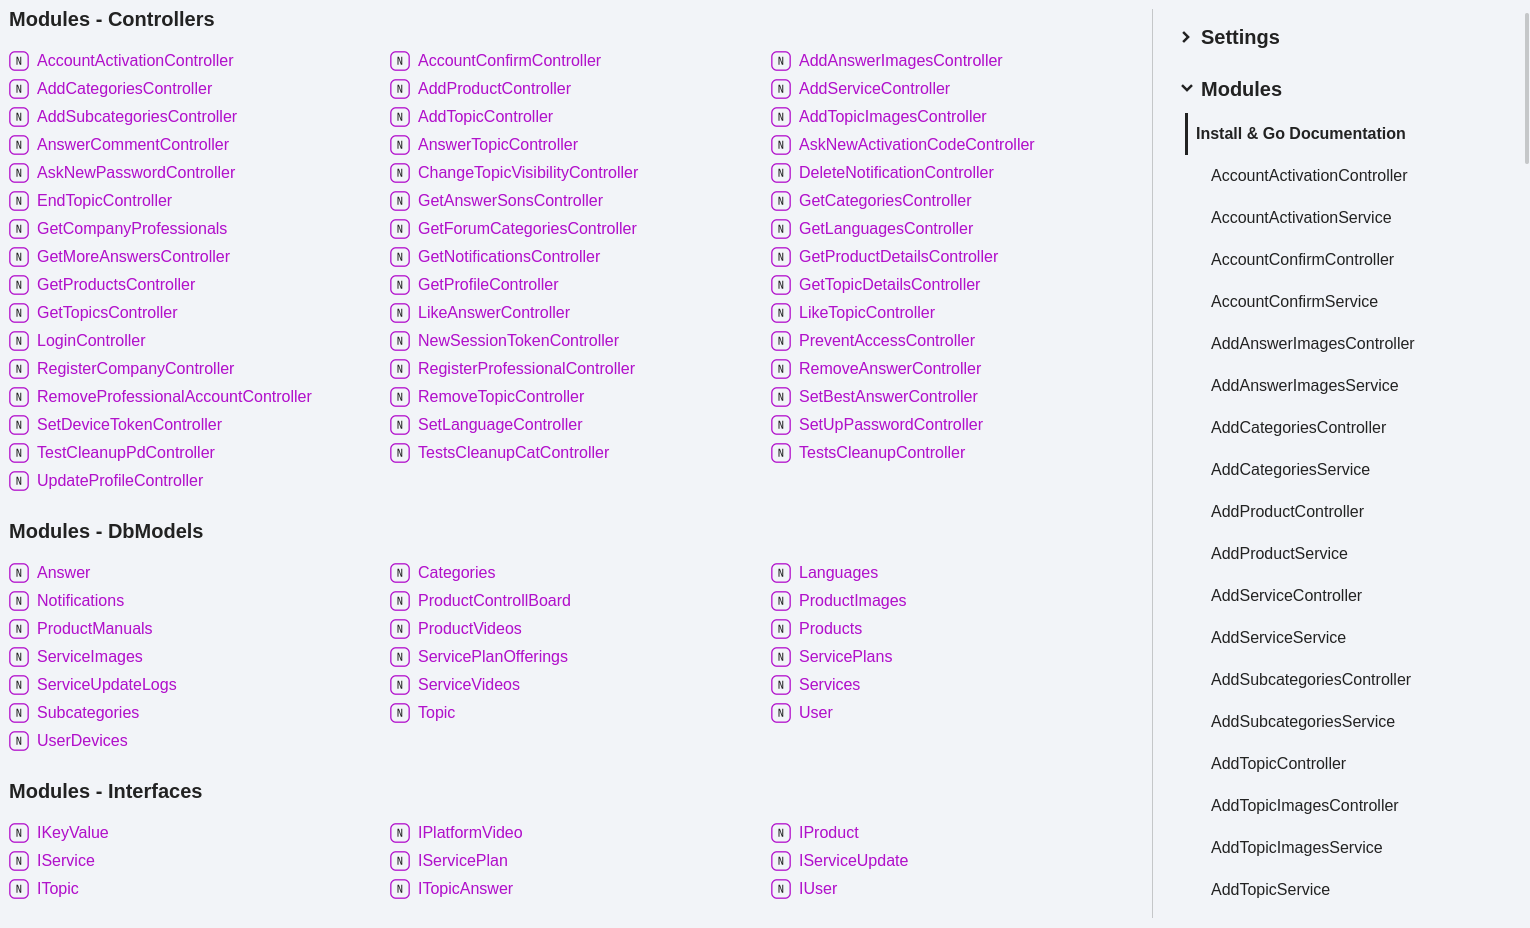
\includegraphics[width=\textwidth]{images/implementacao/api/docs.png}
  \caption{Página inicial da documentação gerada}
  \label{fig:65}
\end{figure}

\newpage

\subsubsection{Swagger}
Swagger é uma ferramenta que permite gerar documentação a nivel de serviços, esta documentação é acessível a partir do mesmo servidor indicando uma rota para o mesmo, evitando assim outro servidor para hospedar a documentação, a base de toda a documentação encontra-se em um ficheiro no formato json. Esta documentação poderá ser gerada a partir de comentários a nivel de código ou a partir de um ficheiro em formato json como mencionado anteriormente. Este ficheiro em formato json poderá ser mantido manualmente ou automaticamente.

Apesar da ferramenta disponibilizar a geração automática de documentação a partir de comentários de código, foram encontrados alguns problemas com esta funcionalidade, acabando por não gerar a documentação, pelo que foi optado por manter a documentação manualmente com o ficheiro json. Esta ferramenta oferece diversas funcionalidades como autenticação, definição de estruturas de dados para os serviços e exemplos de respostas para os mesmos, ambas estas funcionalidades foram exploradas conseguindo assim um bom suporte de documentação para qualquer utilizador.

\begin{figure}[htb]
  \centering
  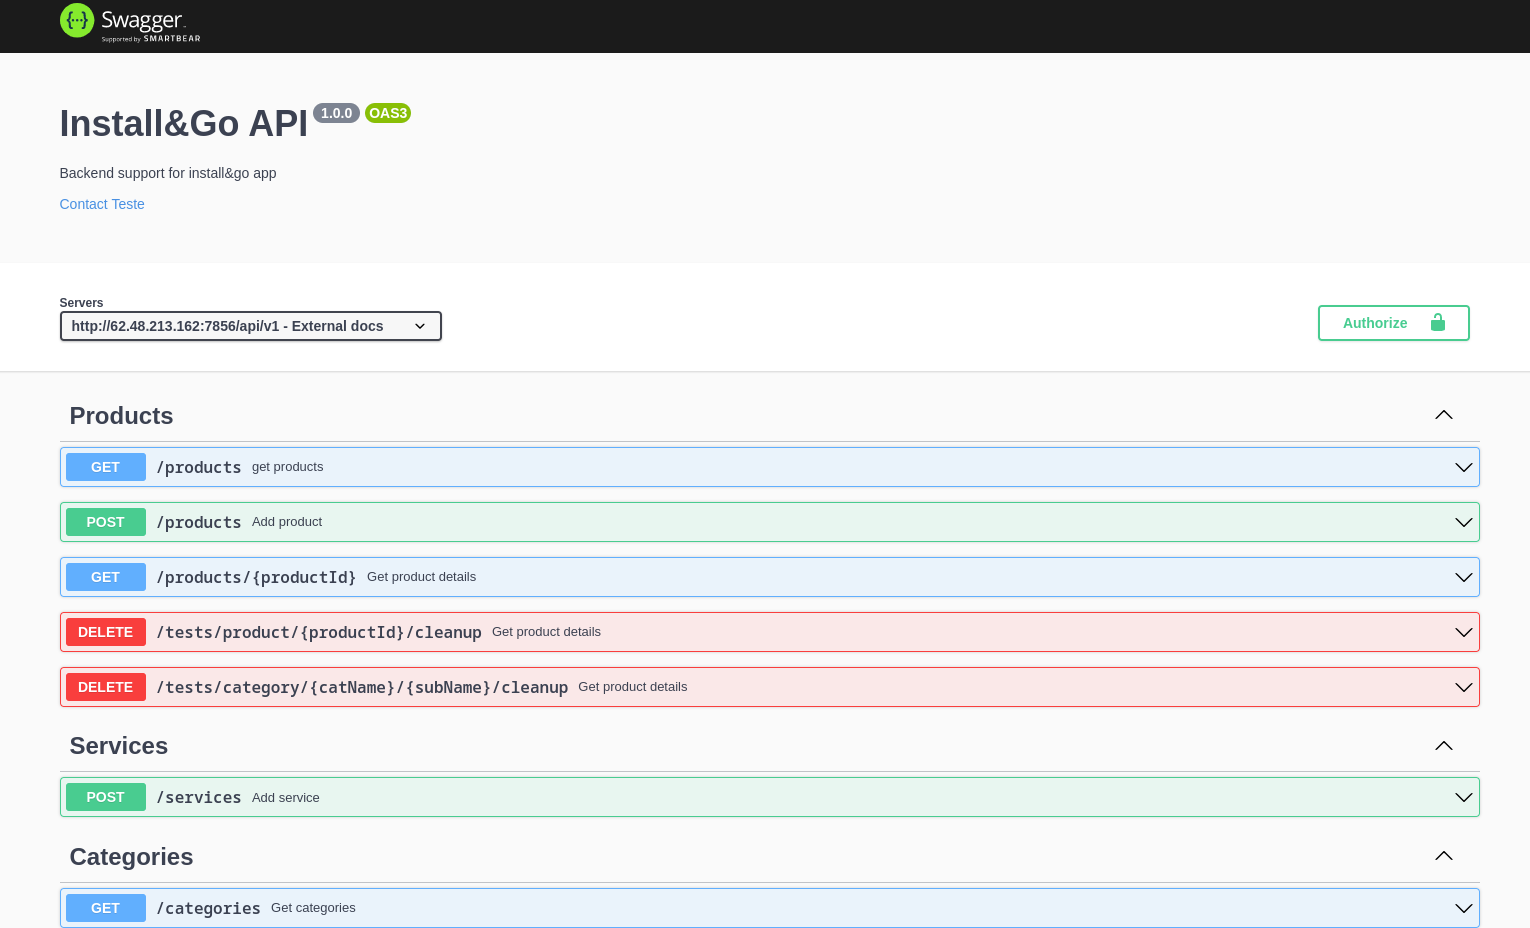
\includegraphics[width=0.6\textwidth]{images/implementacao/api/swagger_intro.png}
  \caption{Documentação swagger}
  \label{fig:66}
\end{figure}

\begin{figure}[htb]
  \centering
  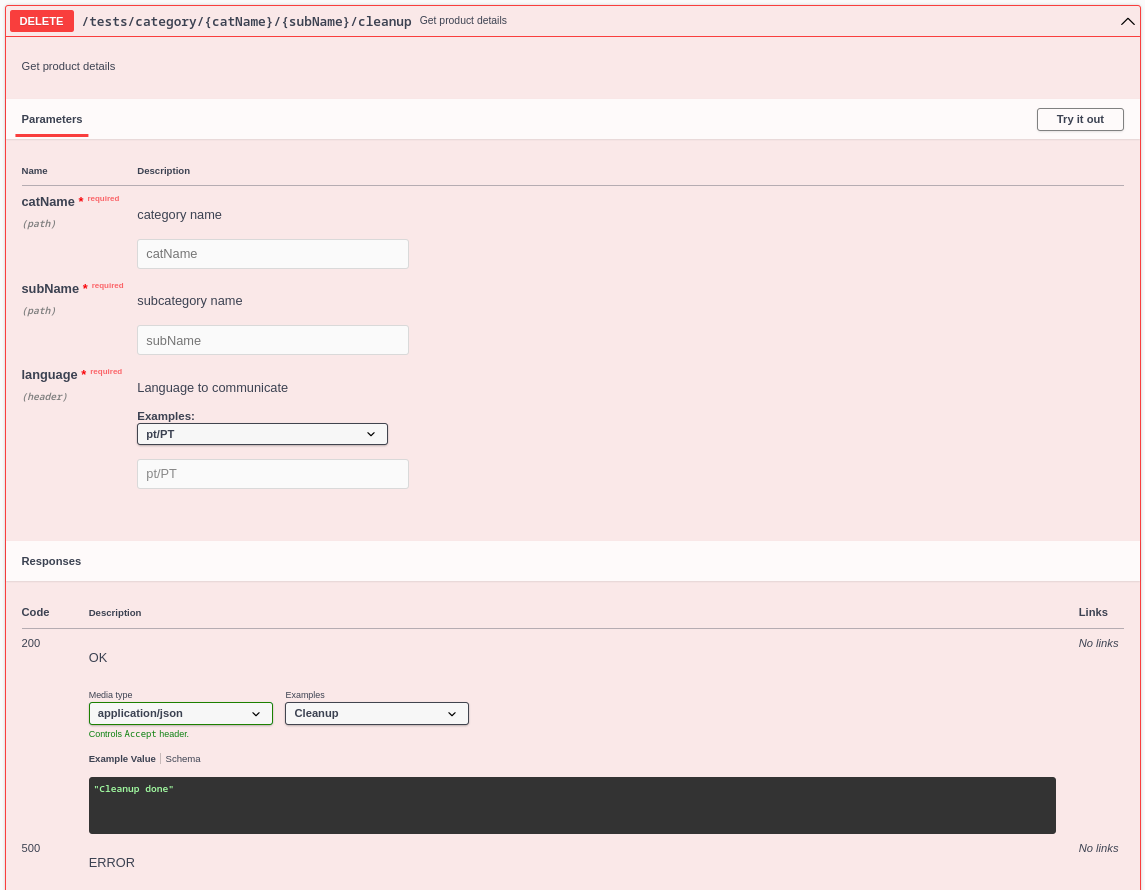
\includegraphics[width=0.6\textwidth]{images/implementacao/api/swagger_pedido.png}
  \caption{Exemplo de documentação de serviço}
  \label{fig:67}
\end{figure}